\documentclass[11pt]{article}
\usepackage[margin=1in]{geometry}
\usepackage[T1]{fontenc}
\usepackage[utf8]{inputenc}
\usepackage{lmodern}
\usepackage{microtype}
\usepackage{amsmath,amssymb,mathtools}
\usepackage{graphicx}
\usepackage{hyperref}
\hypersetup{hidelinks}
\usepackage{parskip}
\usepackage{tikz}
\usepackage{pgfplots}
\usetikzlibrary{arrows.meta,positioning,calc}
\pgfplotsset{compat=1.18}
\setcounter{tocdepth}{3}

\title{Acquisition and Analysis of Neural Data\\Lecture Notes}
\author{}
\date{}

\begin{document}
\maketitle
\tableofcontents

\section{Lecture 1: Spikes (Part 1)}

\subsection{Neural coding: encoding and decoding}

These notes cover the opening lecture of the spike-train block of \emph{Acquisition and Analysis of Neural Data}. The lecture follows the beginning of Chapter 1 of Dayan and Abbott's \emph{Theoretical Neuroscience} and introduces the central problem of the course: how to relate spike trains to stimuli, actions, and internal neural computations.

The broad theme is \emph{neural coding}. A nervous system receives inputs from the world, transforms them through neural circuitry, and produces outputs such as motor commands or decisions. The experimentally accessible signals are often sequences of action potentials, or \emph{spikes}. Understanding which aspects of those spike trains carry information is the starting point for both neural data analysis and theoretical neuroscience.

\subsubsection{Why spikes matter}

Neurons come in a wide range of morphologies and biophysical specializations, but across cell types the action potential is the basic long-range signaling event. In contrast to graded membrane fluctuations, spikes have a remarkably stereotyped waveform once initiated. The lecture emphasized several key properties:
\begin{itemize}
    \item spikes have a nearly uniform shape,
    \item their amplitude is on the order of $100\,\mathrm{mV}$,
    \item their duration is approximately $1\,\mathrm{ms}$,
    \item they are followed by an absolute refractory period of a few milliseconds,
    \item they may also show a longer relative refractory period,
    \item and, unlike passive voltage spread, they can actively propagate over long distances along axons.
\end{itemize}

This stereotypy is both a blessing and a limitation. It is a blessing because spike times can be identified robustly and compared across trials. It is a limitation because, once we reduce neural activity to spike times, much of the subthreshold membrane dynamics is discarded. The coding question therefore becomes: \emph{which statistical features of the spike train should be treated as the neural response?}

\subsubsection{From stimulus to response, and back again}

The lecture framed neural coding through two complementary tasks:
\begin{itemize}
    \item \textbf{Encoding:} given a stimulus $s$, predict the neural response $r$.
    \item \textbf{Decoding:} given a neural response $r$, infer the stimulus $s$.
\end{itemize}

Here the word ``stimulus'' should be interpreted broadly. In sensory systems it may be light intensity, sound pressure, whisker motion, or some richer time-dependent signal. In motor systems it may be a movement direction, force, or behavioral state. Likewise, the response $r$ may be a raw spike train, a firing rate, a population response, or a more structured feature vector derived from spiking activity.

\begin{figure}[h]
\centering
\includegraphics[width=0.9\textwidth]{figures/aand-coding-loop.png}
\caption{The two central directions of neural coding. Encoding models predict responses from stimuli; decoding models infer stimuli or behavioral variables from measured neural activity.}
\end{figure}

This distinction is foundational for the rest of the course. Lectures 1--2 focus mainly on encoding, Lecture 3 turns to decoding, and later lectures add information-theoretic viewpoints.

\subsubsection{Recording neural signals}

The lecture briefly contrasted the main recording modalities relevant to spike analysis.

\paragraph{Intracellular recordings.}
Recording from the soma or axon directly reveals the full membrane potential trajectory, including subthreshold fluctuations and the full spike waveform. This provides rich mechanistic information, but such recordings are technically demanding and often limited to few neurons at a time.

\paragraph{Extracellular recordings.}
When an electrode is placed outside the neuron, the measured voltage deflection is much smaller than the intracellular signal, but spikes can still be detected as transient events. Extracellular recording is therefore the standard route to collecting spike trains from many neurons in vivo. In the lecture, tetrodes were highlighted as an important example: by recording from several nearby contacts simultaneously, one can improve \emph{spike sorting}, i.e. the separation of spikes emitted by different neurons. The lecture also emphasized the strong spatial attenuation of extracellular signals: as a rough rule of thumb, individual spikes are most detectable only within distances on the order of $100\,\mu\mathrm{m}$ from the recording site. This is why electrode spacing matters. To isolate single neurons reliably, contacts typically need to be separated on the order of $150\,\mu\mathrm{m}$ so that nearby cells produce distinguishable signatures across channels; beyond that range, attributing a waveform to one neuron becomes much harder.

\paragraph{Population-level signals.}
The lecture also alluded to larger-scale signals such as EEG, local field potentials (LFP), and multiunit activity (MUA). These are related to neural activity, but they are not equivalent to isolated single-neuron spike trains. Their relationship to spiking becomes especially important once one studies coordinated population activity. EEG in particular reflects the aggregate activity of many neurons recorded from the brain surface, so one should usually not expect to isolate a single neuron from it. Only in special circumstances---for example very long recordings with unusually favorable geometry and electrode placement---can one hope to infer more spatially specific structure from such signals.

\begin{figure}[h]
\centering
\includegraphics[width=0.9\textwidth]{figures/aand-recording-scale.png}
\caption{Intuition for recording scale. Extracellular contacts resolve very local spike sources, while EEG reflects pooled activity from many distant neurons and therefore trades spatial specificity for broad population coverage.}
\end{figure}

\subsection{Spike trains as mathematical objects}

To analyze spikes quantitatively, we need a representation that is precise enough for mathematics but still close to the data. The lecture introduced the standard point-process description.

\subsubsection{Spike times and the neural response function}

Suppose a neuron emits spikes at times
\[
\{t_1,t_2,\dots,t_n\}, \qquad 0 \le t_i \le T,
\]
within an observation window of duration $T$. The corresponding neural response function is written as
\[
\rho(t) = \sum_{i=1}^{n} \delta(t-t_i),
\]
where $\delta$ denotes the Dirac delta.

This notation is extremely useful. It packages an entire spike train into a single object while preserving exact spike timing. The response function $\rho(t)$ is not an ordinary function in the classical sense; rather, it is a generalized function or distribution. Informally, it is zero everywhere except at spike times, yet its integral over a region counts spikes in that region.

\subsubsection{The role of the Dirac delta}

The lecture used a heuristic representation of the delta function as a limit of narrower and taller rectangles. Formally, the object is best characterized by its defining properties:
\begin{align*}
\delta(\tau) &= 0 \quad \text{for } \tau \ne 0,\\
\int_{-\infty}^{\infty} \delta(\tau)\,d\tau &= 1,\\
\int_a^b \delta(t-\tau)h(\tau)\,d\tau &=
\begin{cases}
 h(t), & a<t<b,\\
 0, & \text{otherwise.}
\end{cases}
\end{align*}
The last identity is the \emph{sifting property}; it expresses that integrating against a delta picks out the value of the function at the spike time.

For spike trains this gives an immediate interpretation:
\[
\int_a^b \rho(t)\,dt = \text{number of spikes in } [a,b].
\]
So $\rho$ is the mathematically clean object from which various notions of firing rate can be derived.

\subsection{Why introduce a firing rate?}

A single spike train is a set of discrete events in time, whereas many stimuli of interest are continuous and time-varying. This mismatch motivates the introduction of a smoother response descriptor. The lecture's answer is the \emph{firing rate}: a rate-like quantity obtained by averaging the spike train in time, across trials, across neurons, or by combinations of these operations.

Raster plots make the need for averaging visually obvious. Repeated presentations of the same stimulus often elicit similar response structure, but with considerable trial-to-trial variability. A rate estimate summarizes that structure while suppressing microscopic irregularities.

At the same time, the lecture stressed an important conceptual warning: there is \emph{no unique firing rate hidden inside a finite dataset}. Different averaging procedures produce different rate estimates, each with different biases and interpretations.

\subsection{Temporal averaging of a single spike train}

\subsubsection{Binning}

The simplest construction divides time into bins of width $\Delta t$. If $n_k$ is the number of spikes in bin $k$, then the binned firing rate is
\[
r(k\Delta t) := \frac{n_k}{\Delta t}
= \frac{1}{\Delta t}\int_{k\Delta t}^{(k+1)\Delta t} \rho(\tau)\,d\tau.
\]
This is often the first rate estimate one computes in practice.

A special case is obtained by setting the bin width equal to the full trial length, $\Delta t = T$. Then one obtains the \emph{spike count rate}
\[
r = \frac{1}{T}\int_0^T \rho(\tau)\,d\tau = \frac{n}{T}.
\]
This quantity ignores all temporal structure within the trial and keeps only the total spike count per unit time.

Binning is simple and intuitive, but it has two limitations already emphasized in the lecture:
\begin{itemize}
    \item the resulting rate takes discrete values, because spike counts are integers,
    \item and the estimate depends on the arbitrary placement of bin boundaries.
\end{itemize}
A spike that falls just to the left or right of a bin edge can change the binned curve substantially.

\subsubsection{Linear filtering}

A more flexible alternative is to smooth the spike train with a normalized kernel $w$:
\[
r(t) := \int_{-\infty}^{\infty} w(\tau)\,\rho(t-\tau)\,d\tau,
\qquad
\int_{-\infty}^{\infty} w(\tau)\,d\tau = 1.
\]
Substituting $\rho(t)=\sum_i \delta(t-t_i)$ gives
\[
r(t)=\sum_{i=1}^{n} w(t-t_i).
\]
Thus, linear filtering turns the spike train into a sum of shifted kernel shapes, one centered on each spike time.

This is one of the most useful formulas in the lecture. It says that a firing-rate estimate is not something mysterious; it is simply what results when each spike is replaced by a small template and all templates are added together.

\subsubsection{Common kernel choices}

\paragraph{Rectangular kernel.}
A sliding-window or running-average estimate uses
\[
w(\tau)=
\begin{cases}
\dfrac{1}{\Delta t}, & -\dfrac{\Delta t}{2} < \tau < \dfrac{\Delta t}{2},\\[6pt]
0, & \text{otherwise.}
\end{cases}
\]
Compared with fixed binning at the same width $\Delta t$, this avoids arbitrary bin alignment because the window moves continuously with time. However, the resulting values are still piecewise constant, neighboring times become correlated, and the kernel is noncausal because it depends on future spikes as well as past ones.

\paragraph{Gaussian kernel.}
A smooth rate estimate is obtained from
\[
w(\tau)=\frac{1}{\sqrt{2\pi}\,\sigma_w}
\exp\!\left(-\frac{\tau^2}{2\sigma_w^2}\right).
\]
This produces a continuous and visually appealing rate curve. The trade-off is that the estimate remains noncausal and again introduces temporal correlations by construction.

\paragraph{Alpha kernel.}
A causal alternative is the alpha-function kernel
\[
w(\tau)=\bigl[\alpha^2 \tau e^{-\alpha \tau}\bigr]_+,
\qquad
[z]_+ =
\begin{cases}
z, & z\ge 0,\\
0, & z<0.
\end{cases}
\]
Unlike the rectangular and Gaussian kernels, this filter vanishes for negative times and therefore depends only on present and past spikes. It is closer to causal synaptic filtering, but it is biased toward positive times because each spike contributes only after it occurs. In practical use, the lecture suggested choosing the characteristic timescale $\alpha^{-1}$ on the order of $10$--$15\,\mathrm{ms}$ as a reasonable causal smoothing window, while still relating the final choice to the mean interspike interval of the neuron under study.

\subsubsection{Bias-variance trade-off in rate estimation}

The lecture summarized the main trade-off succinctly:
\begin{itemize}
    \item narrower kernels give higher temporal resolution,
    \item wider kernels give lower variability.
\end{itemize}
In symbols, smaller $\Delta t$, smaller $\sigma_w$, or larger $\alpha$ preserve faster changes but make the estimate noisier; broader kernels smooth more strongly but can wash out real temporal structure.

A useful rough lower bound for kernel width is the mean interspike interval,
\[
\frac{T}{n}.
\]
If one smooths on a much shorter timescale than the typical spacing between spikes, the resulting ``rate'' largely reflects the discreteness of single spikes rather than a stable underlying trend.

\begin{figure}[h]
\centering
\includegraphics[width=0.9\textwidth]{figures/aand-rate-estimation.png}
\caption{Rate-estimation trade-off. Narrow kernels preserve fast changes but amplify variability, whereas broader kernels produce more stable firing-rate estimates at the cost of temporal precision.}
\end{figure}

\begin{figure}[h]
\centering
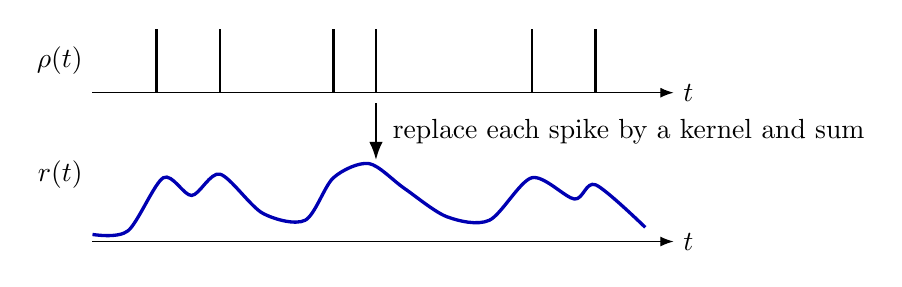
\begin{tikzpicture}[x=0.9cm,y=0.9cm,>=Latex]
    % Spike train axis
    \draw[->] (0,0) -- (8.2,0) node[right] {$t$};
    \foreach \x in {0.9,1.8,3.4,4.0,6.2,7.1} {
        \draw[line width=0.9pt] (\x,0) -- (\x,0.9);
    }
    \node[left] at (0,0.45) {$\rho(t)$};

    % Smoothed trace
    \draw[->] (0,-2.1) -- (8.2,-2.1) node[right] {$t$};
    \node[left] at (0,-1.15) {$r(t)$};
    \draw[very thick, blue!70!black, smooth] plot coordinates {
        (0.0,-2.0) (0.5,-1.95) (1.0,-1.2) (1.4,-1.45) (1.8,-1.15)
        (2.4,-1.7) (3.0,-1.8) (3.4,-1.2) (3.9,-1.0) (4.4,-1.35)
        (5.0,-1.75) (5.6,-1.8) (6.2,-1.2) (6.8,-1.5) (7.1,-1.3) (7.8,-1.9)
    };
    \draw[->,thick] (4.0,-0.15) -- (4.0,-0.95);
    \node[right] at (4.1,-0.55) {replace each spike by a kernel and sum};
\end{tikzpicture}
\caption{Schematic view of temporal averaging. The spike train $\rho(t)$ is converted into a rate estimate $r(t)$ by replacing each spike with a kernel and summing the resulting contributions.}
\end{figure}

\subsubsection{What temporal averaging changes}

Temporal smoothing is not an innocent visualization step. It changes the statistics of the data. In particular, smoothing introduces artificial temporal correlations: nearby values of $r(t)$ are similar partly because the same spikes contribute to both. This is why one must interpret smoothed rates with care, especially when making claims about temporal precision or causality.

\subsection{Trial averaging}

Temporal smoothing is not the only way to average. When the same stimulus is presented repeatedly, one can average across trials.

If $\rho_k(t)$ denotes the response on trial $k$ and there are $N$ trials, the trial-averaged response function is
\[
\langle \rho(t) \rangle := \frac{1}{N}\sum_{k=1}^{N} \rho_k(t).
\]
This quantity is mathematically well defined, but by itself it is still a sum of delta functions and therefore does not become a smooth ordinary function. Summing spike trains across trials and dividing by $N$ still leaves an aggregate point process rather than a directly interpretable rate curve. For that reason, the lecture emphasized that $\langle \rho(t) \rangle$ alone is usually not the final object of interest.

\subsubsection{Trial average combined with temporal averaging}

A practically useful quantity is obtained by averaging across trials and then smoothing in time. Using a rectangular window of width $\Delta t$ gives
\[
\langle r(t) \rangle := \frac{1}{\Delta t}
\int_t^{t+\Delta t} \langle \rho(\tau) \rangle\,d\tau.
\]
This is the trial-averaged, time-dependent firing rate. Operationally, one can think of this as sliding a small rectangular window across the aggregated response function and counting how much spike mass falls into each window. With sufficiently small bins, this produces a granular but much more interpretable description of how firing rate evolves over time.

Because averaging has already reduced variability across trials, one can often choose much smaller temporal windows than for a single-trial estimate. This is one reason why peristimulus time histograms and related averages are so informative in sensory neuroscience.

A further special case is the average firing rate over the whole trial:
\[
\langle r \rangle := \frac{\langle n \rangle}{T}
= \frac{1}{T}\int_0^T \langle \rho(\tau) \rangle\,d\tau.
\]
This scalar summarizes how strongly the neuron responds on average under a fixed stimulus condition.

\subsubsection{Interpreting $\langle r(t) \rangle$}

The lecture gave two especially important interpretations.

\paragraph{Expected spike count.}
The total area under the rate curve over an interval estimates the expected number of spikes in that interval:
\[
\int_a^b \langle r(t) \rangle\,dt \approx \text{expected spike count on } [a,b].
\]
Over the full trial this becomes the mean number of spikes per trial.

\paragraph{Approximate spike probability in a short window.}
If the interval $[t_a,t_b]$ is short enough that the expected spike count is much smaller than $1$, then
\[
\int_{t_a}^{t_b} \langle r(t) \rangle\,dt
\approx \langle r(t_a) \rangle (t_b-t_a)
\]
can be interpreted as the probability of observing a spike in that window on a given trial.

This local probabilistic interpretation explains why firing rates are so useful in encoding models: a time-dependent rate can be viewed as the intensity of an inhomogeneous point process.

\subsubsection{What a firing rate does not tell you}

The lecture illustrated that the same time-dependent mean rate can arise from qualitatively different single-trial statistics. For example, spikes might appear nearly independent across trials, or they might be clustered or otherwise interdependent within a trial. In both cases the averaged curve $\langle r(t) \rangle$ could look very similar.

A useful classroom example is a raster in which each trial contains a single spike and those spikes are spread rather evenly across the observation window. By eye, one may be tempted to say that the neuron has a constant firing tendency and that nothing suggests temporal clustering. But this kind of visual impression is not, by itself, evidence for independence. The lecture explicitly raised the question of how one would justify such a claim quantitatively rather than rhetorically.

So a firing rate captures the first-order tendency to spike, but not the full structure of variability. Later analyses therefore need tools beyond rate curves alone, such as interval statistics, count variability, correlations, and explicit stochastic spike-train models. In particular, one wants statistics that compare variability across trials to what would be expected under an independent-spiking model. Spike-count variance, Fano factors, interspike-interval structure, or cross-trial correlation analyses are examples of the kinds of measures needed to move from visual inspection to defensible inference.

\subsection{Averaging across neurons}

The lecture also introduced a third kind of averaging: averaging over neurons rather than over time or repeated presentations.

If $\rho^{\mathrm{neuron}}_m(t)$ is the response of neuron $m$ among $M$ recorded neurons, then the neuron-averaged response is
\[
\langle \rho(t) \rangle_{\mathrm{neuron}} :=
\frac{1}{M}\sum_{m=1}^{M} \rho^{\mathrm{neuron}}_m(t).
\]
Applying temporal smoothing then gives a neuron-averaged, time-dependent firing rate,
\[
\langle r(t) \rangle_{\mathrm{neuron}} :=
\frac{1}{\Delta t}\int_t^{t+\Delta t} \langle \rho(\tau) \rangle_{\mathrm{neuron}}\,d\tau.
\]
As with trial averaging, averaging over many neurons can justify using relatively small temporal windows because stochastic variability is reduced by pooling.

\subsubsection{The independence caveat}

The lecture's auditory-cortex example made the central caution explicit: neurons are generally \emph{not} independent. If neurons are recorded in different trials and then averaged together, the result does not automatically reconstruct what a simultaneously active population would have done in a single trial.

This matters because correlated population activity can reflect common input, shared network state, oscillations, or stimulus-locked structure. The lecture connected this to the relation between spiking, local field potentials, and multiunit activity. Population codes therefore require more than simply averaging isolated single-neuron recordings gathered under superficially similar conditions.

\subsection{Summary of rate concepts introduced in the lecture}

The lecture used the term ``firing rate'' in several related but non-identical senses. It is useful to keep them distinct:

\begin{center}
\begin{tabular}{ll}
\hline
Quantity & Interpretation \\
\hline
$\rho(t)$ & exact spike train as a sum of deltas \\
$r(t)$ & temporally smoothed single-trial rate estimate \\
$r$ & spike count rate $n/T$ on one trial \\
$\langle r(t) \rangle$ & trial-averaged, time-dependent firing rate \\
$\langle r \rangle$ & mean firing rate across the whole trial \\
$\langle r(t) \rangle_{\mathrm{neuron}}$ & neuron-averaged rate estimate \\
\hline
\end{tabular}
\end{center}

Two conceptual conclusions from the lecture are worth making explicit:
\begin{enumerate}
    \item There is no unique ``true firing rate'' that can be read off from finitely many noisy observations without modeling assumptions.
    \item Any particular rate estimate reflects the averaging operation used to define it. The estimate is therefore useful only when its construction matches the scientific question.
\end{enumerate}

\subsection{Tuning curves as the simplest encoding model}

After introducing firing rates, the lecture moved to the simplest kind of encoding relationship: the dependence of average firing rate on a constant stimulus parameter.

If the stimulus is held fixed at a value $s$, then one may summarize the neural response by the average firing rate $\langle r \rangle$. An encoding model then specifies a function
\[
\langle r \rangle = f(s),
\]
called a \emph{tuning curve}. Here $s$ is one-dimensional, such as orientation, sound frequency, movement direction, or another scalar experimental parameter.

Tuning curves are deliberately low-dimensional summaries. They ignore trial-to-trial fluctuations and much of the temporal structure of spike trains, but they are often the right starting point for characterizing what variable a neuron is sensitive to.

\subsubsection{Gaussian tuning curves}

In visual cortex, some neurons respond preferentially to a particular stimulus value and decrease their firing as the stimulus moves away from that preferred value. A common idealized form is the Gaussian tuning curve,
\[
f(s)=r_0 + A\exp\!\left(-\frac{(s-s_0)^2}{2\sigma^2}\right),
\]
where $r_0$ is a baseline rate, $A$ is the response amplitude, $s_0$ is the preferred stimulus, and $\sigma$ controls tuning width.

The shape expresses a simple encoding principle: the neuron is most active near its preferred feature value and less active for dissimilar inputs.

\subsubsection{Cosine tuning curves}

In motor cortex, directional responses are often approximated by a cosine,
\[
f(\theta)=r_0 + A\cos(\theta-\theta_0),
\]
where $\theta_0$ is the preferred movement direction.

Cosine tuning is especially convenient because it connects naturally to vector representations of movement direction and to population-vector decoding ideas developed later in the literature.

\begin{figure}[h]
\centering
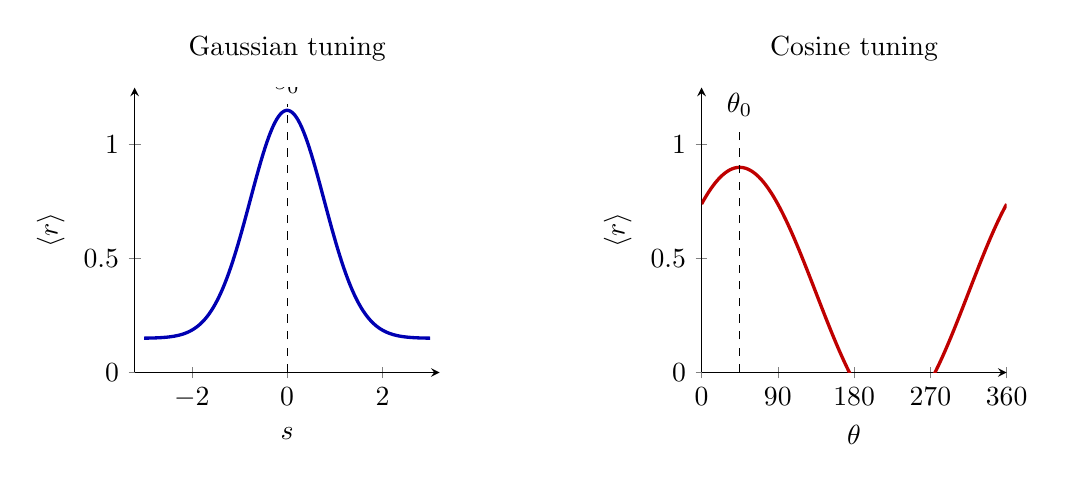
\begin{tikzpicture}
\begin{axis}[
    width=0.45\textwidth,
    height=5.2cm,
    xmin=-3.2,xmax=3.2,
    ymin=0,ymax=1.25,
    axis lines=left,
    xlabel={$s$},
    ylabel={$\langle r \rangle$},
    title={Gaussian tuning},
    samples=150,
    domain=-3:3,
    xtick={-2,0,2},
    ytick={0,0.5,1.0}
]
\addplot[very thick,blue!70!black] {0.15 + exp(-x^2/1.2)};
\draw[dashed] (axis cs:0,0) -- (axis cs:0,1.18);
\node[anchor=south] at (axis cs:0,1.18) {$s_0$};
\end{axis}
\begin{axis}[
    at={(7.2cm,0)},
    anchor=south west,
    width=0.45\textwidth,
    height=5.2cm,
    xmin=0,xmax=360,
    ymin=0,ymax=1.25,
    axis lines=left,
    xlabel={$\theta$},
    ylabel={$\langle r \rangle$},
    title={Cosine tuning},
    samples=200,
    domain=0:360,
    xtick={0,90,180,270,360},
    ytick={0,0.5,1.0}
]
\addplot[very thick,red!75!black] {0.35 + 0.55*cos(x-45)};
\draw[dashed] (axis cs:45,0) -- (axis cs:45,1.08);
\node[anchor=south] at (axis cs:45,1.08) {$\theta_0$};
\end{axis}
\end{tikzpicture}
\caption{Two canonical tuning-curve shapes emphasized in the lecture: Gaussian tuning, often used for sensory selectivity, and cosine tuning, often used for directional motor responses.}
\end{figure}

\subsection{Conceptual takeaways from Lecture 1}

The first lecture established the language used throughout the rest of the spike-train unit.

\begin{itemize}
    \item Spikes are treated as the elementary signaling events of neural communication.
    \item A spike train can be represented exactly as $\rho(t)=\sum_i \delta(t-t_i)$.
    \item Firing rates are not primitive observables but averaged versions of spike trains.
    \item Different averaging procedures---over time, trials, or neurons---serve different scientific purposes and impose different assumptions.
    \item A time-dependent firing rate can often be interpreted as an expected spike count density, but it does not by itself capture higher-order spike statistics or dependencies.
    \item Tuning curves provide the simplest link between stimuli and average firing rates and therefore the simplest example of an encoding model.
\end{itemize}

These ideas will support the next steps in the course: understanding spike-train variability more explicitly, constructing richer encoding models, and ultimately asking how stimuli or movements can be decoded from neural activity.

\subsection*{Sources mentioned in Lecture 1}

\begin{itemize}
    \item P. Dayan and L. F. Abbott (2001), \emph{Theoretical Neuroscience: Computational and Mathematical Modeling of Neural Systems}. MIT Press.
    \item A. Luczak, P. B. Barto, and K. D. Harris (2013), experimental examples on population activity in auditory cortex discussed in the lecture slides.
    \item G. Buzs\'aki (2004), extracellular recording and tetrode context discussed in the lecture slides.
\end{itemize}

\clearpage
\section{Lecture 2: Time-dependent encoding and spike-train statistics}

Lecture 1 introduced the simplest encoding picture: a constant stimulus parameter mapped to an average firing rate through a tuning curve. Lecture 2 generalizes that picture to \emph{time-dependent stimuli} and \emph{time-dependent firing rates}. The central question becomes: if a neuron emits a spike at time $t_i$, what was the stimulus doing shortly before that spike, and what statistical structure of the spike train is needed to answer that question rigorously?

The lecture pursued this question in two linked steps. First, it introduced the \emph{spike-triggered average} (STA), which summarizes the typical stimulus pattern preceding spikes and thereby connects encoding to reverse-correlation methods. Second, it shifted from rate descriptions alone to explicit \emph{spike-train statistics}, using the homogeneous Poisson process as the simplest tractable probabilistic model.

\subsection{From static tuning curves to time-dependent encoding}

The conceptual move from Lecture 1 to Lecture 2 is easy to state but important to internalize:
\begin{itemize}
    \item for static or slowly varying conditions, one often writes an encoding relation of the form
    \[
    s \mapsto \langle r \rangle,
    \]
    where a fixed stimulus value is associated with an average firing rate;
    \item for genuinely time-varying stimuli, the natural object is instead
    \[
    s(t) \mapsto \langle r(t) \rangle.
    \]
\end{itemize}

This is a much richer problem. The neuron is no longer characterized only by which stimulus value it prefers; one also wants to know \emph{which temporal patterns} of the stimulus tend to precede spiking. In other words, one is now asking about a neuron's temporal receptive field rather than only about a static tuning curve.

\subsection{The spike-triggered average}

\subsubsection{Definition and intuition}

Suppose a spike train contains spike times $t_1,\dots,t_n$ during an observation window, and suppose a time-dependent stimulus $s(t)$ is presented during that same window. The spike-triggered average is defined by averaging the stimulus trace at a fixed temporal lag before each spike:
\[
C(\tau) := \left\langle \frac{1}{n}\sum_{i=1}^{n} s(t_i-\tau)\right\rangle .
\]
Here $\langle \cdot \rangle$ denotes an average over repeated trials or repetitions of the same stimulus condition.

In the lecture, this definition was paired with a useful simplifying assumption:
\[
\int_0^T s(t)\,dt = 0.
\]
The motivation is physiological as well as mathematical. Sensory systems often adapt to the \emph{average} stimulus intensity, so the interesting part of the drive is the fluctuation around baseline rather than the baseline itself. If one did not remove the mean, then the STA would inherit a trivial constant offset that says little about which \emph{time-dependent feature} actually drives spikes.

The sign convention matters. The argument $t_i-\tau$ means that positive $\tau$ corresponds to looking \emph{backward in time} from the spike. Thus, $C(\tau)$ answers the question:
\begin{quote}
What did the stimulus typically look like $\tau$ milliseconds before a spike occurred?
\end{quote}

Operationally, the computation is simple:
\begin{enumerate}
    \item take each spike time as an alignment point,
    \item cut out a short window of stimulus values preceding that spike,
    \item align these stimulus snippets at the spike,
    \item and average them.
\end{enumerate}

The result is a typical pre-spike stimulus waveform. If the neuron is systematically driven by some particular stimulus pattern, that structure should appear in the STA.

\subsubsection{What the STA is trying to reveal}

The STA is useful because it compresses a potentially complicated stimulus-response relationship into an interpretable time course. Instead of asking for the full joint distribution of stimulus histories and spike trains, one asks for the average stimulus history conditioned on spiking. The method is therefore especially attractive as a first pass at identifying which stimulus features matter for firing.

The lecture emphasized that the STA is an \emph{encoding} tool. It does not tell us what information the neuron ultimately transmits to a downstream observer. Rather, it characterizes what kinds of stimulus fluctuations tend to drive the neuron strongly enough to produce spikes.

\subsubsection{Expected qualitative features}

Several qualitative properties of $C(\tau)$ were highlighted:
\begin{itemize}
    \item for large positive lags, $C(\tau)$ should often decay back toward baseline, reflecting the neuron's finite memory;
    \item for sufficiently negative lags, one expects no causal influence of the future stimulus on a past spike;
    \item if spikes are statistically unrelated to the stimulus, the STA should be close to zero at all lags.
\end{itemize}

The second point deserves care. In ideal causal systems, future stimulus values should not predict past spikes. But the lecture noted that one can still observe nonzero STA values at small negative lags. This does \emph{not} imply that the neuron anticipates the future. Instead, it often reflects \emph{stimulus autocorrelation}: if nearby stimulus samples are correlated with one another, a response to the recent past can spill into apparently post-spike stimulus averages.

\subsubsection{Examples from sensory and population recordings}

The slide deck showed several examples illustrating that STA is not tied to a single modality:
\begin{itemize}
    \item electrosensory neurons in weakly electric fish,
    \item the blowfly H1 neuron responding to visual motion,
    \item and even spike-triggered EEG analyses in contemporary systems neuroscience.
\end{itemize}

These examples are pedagogically useful because they show both the strength and the limitation of the STA. The strength is that one often obtains a clear, biologically meaningful stimulus template from seemingly noisy data. The limitation is that the result depends strongly on the stimulus ensemble and on what kind of spike event is used as a trigger.

\subsection{STA as a reverse-correlation method}

\subsubsection{From spike sums to stimulus-response correlations}

The lecture derived an important approximation that connects the STA to standard correlation functions. Starting from the definition above, one can rewrite the spike sum using the response function
\[
\rho(t)=\sum_{i=1}^{n}\delta(t-t_i),
\]
which gives
\[
\sum_{i=1}^{n} s(t_i-\tau) = \int_0^T \rho(t)\,s(t-\tau)\,dt.
\]
After averaging across trials and replacing $n$ by its trial-averaged value $\langle n \rangle$ for sufficiently large spike counts, one obtains
\[
C(\tau) \approx \frac{1}{\langle n \rangle}\int_0^T \langle \rho(t)\rangle s(t-\tau)\,dt.
\]

Using the same small-bin argument from Dayan and Abbott that appeared in the slides, $\langle \rho(t)\rangle$ inside the integral can be interpreted as the time- and trial-averaged firing rate $\langle r(t)\rangle$. Hence
\[
C(\tau) \approx \frac{1}{\langle n \rangle}\int_0^T \langle r(t)\rangle s(t-\tau)\,dt.
\]

\subsubsection{Detour: why $\langle \rho(t)\rangle$ becomes $\langle r(t)\rangle$ inside the integral}

This replacement is easy to accept formally and easy to forget conceptually, so it is worth unpacking. Divide the observation window into $M\gg 1$ small bins of width $\Delta t$ with grid points $t_m=m\Delta t$. Assuming the stimulus is smooth enough on that scale and identical across trials, one may approximate
\[
\int_0^T \langle \rho(t)\rangle s(t-\tau)\,dt
\approx
\sum_{m=1}^{M} s(t_m-\tau)
\int_{t_{m-1}}^{t_m} \langle \rho(t)\rangle\,dt.
\]
But by the same definition used earlier for time- and trial-averaged firing rates,
\[
\langle r(t_m)\rangle\,\Delta t
:=
\int_{t_{m-1}}^{t_m} \langle \rho(t)\rangle\,dt.
\]
Therefore
\[
\int_0^T \langle \rho(t)\rangle s(t-\tau)\,dt
\approx
\sum_{m=1}^{M} \Delta t\,\langle r(t_m)\rangle s(t_m-\tau),
\]
and this Riemann sum converges back to
\[
\int_0^T \langle r(t)\rangle s(t-\tau)\,dt.
\]
So the lecture's replacement is not mysterious: inside an integral over time, the averaged spike train and the averaged firing rate represent the same spike mass once one coarse-grains at sufficiently fine temporal resolution.

\subsubsection{Cross-correlation and the meaning of the minus sign}

The lecture then introduced the cross-correlation of two signals $x$ and $y$:
\[
Q_{xy}(\tau) := \frac{1}{T}\int_0^T x(t)\,y(t+\tau)\,dt.
\]
Applied to the firing rate and the stimulus, this becomes
\[
Q_{rs}(\tau) := \frac{1}{T}\int_0^T \langle r(t)\rangle s(t+\tau)\,dt.
\]

Comparing this definition with the STA formula yields
\[
C(\tau) = \frac{T}{\langle n \rangle} Q_{rs}(-\tau)
       = \frac{Q_{rs}(-\tau)}{\langle r \rangle},
\]
because $\langle r \rangle = \langle n \rangle / T$.

This identity is conceptually important. The STA is not just an ad hoc average; it is a \emph{reverse correlation}. The minus sign in the argument, $Q_{rs}(-\tau)$, reflects that one aligns the stimulus \emph{before} the spike rather than after it. That is why the method is often described as reverse-correlation analysis in sensory neuroscience.

\subsubsection{Mathematical aside: how to read a correlation function}

The lecture's correlation functions are \emph{raw} lagged overlaps rather than normalized Pearson correlations. That choice is deliberate. The factor $1/T$ keeps the physical units explicit and makes the STA derivation algebraically clean. If one wanted a centered covariance instead, one would replace $x(t)$ and $y(t)$ by $x(t)-\bar{x}$ and $y(t)-\bar{y}$, but the geometric interpretation would stay the same.

For each lag $\tau$, the quantity
\[
Q_{xy}(\tau)=\frac{1}{T}\int_0^T x(t)\,y(t+\tau)\,dt
\]
compares one signal with a shifted copy of the other. Large positive values mean that peaks in $x$ tend to line up with peaks in the shifted $y$; negative values mean that peaks in one signal tend to line up with troughs in the other. The special case
\[
Q_{xx}(0)=\frac{1}{T}\int_0^T x(t)^2\,dt \ge 0
\]
is the average signal power, and for real-valued signals the autocorrelation is an even function:
\[
Q_{xx}(\tau)=Q_{xx}(-\tau).
\]

This overlap viewpoint is the easiest way to remember the STA sign convention. Positive $\tau$ in $C(\tau)$ means ``look earlier than the spike,'' whereas positive $\tau$ in $Q_{rs}(\tau)$ shifts the stimulus forward inside the integral. The relation
\[
C(\tau)=\frac{Q_{rs}(-\tau)}{\langle r \rangle}
\]
simply translates between these two bookkeeping conventions.

\begin{figure}[h]
\centering
\includegraphics[width=\textwidth]{figures/aand-correlation-lagged-overlap.png}
\caption{Lagged-overlap view of the cross-correlation $Q_{xy}(\tau)$. The value at each lag depends on how well one waveform matches a shifted version of the other. In the STA formula, the minus sign appears because one asks for the stimulus \emph{before} the spike rather than after it.}
\end{figure}

\subsubsection{Autocorrelation and why the stimulus ensemble matters}

The lecture also reviewed the autocorrelation of a signal:
\[
Q_{xx}(\tau) := \frac{1}{T}\int_0^T x(t)\,x(t+\tau)\,dt.
\]
For the stimulus itself this gives
\[
Q_{ss}(\tau) := \frac{1}{T}\int_0^T s(t)\,s(t+\tau)\,dt.
\]

This matters because the STA does \emph{not} depend only on the neuron. It also depends on the stimulus statistics. If the stimulus contains strong temporal correlations, then the STA can be broadened or distorted by those correlations. That is the deeper reason why one must choose the stimulus ensemble carefully when estimating receptive fields.

To see the mechanism more concretely, consider the simplified linear-encoding picture
\[
\langle r(t) \rangle = \int_{-\infty}^{\infty} k(u)\,s(t-u)\,du,
\]
where $k$ is the temporal filter one would ideally like to recover. Substituting this into the definition of $Q_{rs}$ gives
\[
Q_{rs}(\tau)=\int_{-\infty}^{\infty} k(u)\,Q_{ss}(\tau+u)\,du.
\]
So the stimulus-response correlation is the neuronal filter blurred by the stimulus autocorrelation. If the stimulus were ideal white noise with
\[
Q_{ss}(\tau)=\sigma_s^2\delta(\tau),
\]
then the blur would collapse to
\[
Q_{rs}(\tau)=\sigma_s^2 k(-\tau),
\]
and therefore
\[
C(\tau)=\frac{\sigma_s^2}{\langle r \rangle}k(\tau).
\]
This is the cleanest mathematical reason white noise is so useful: under the lecture's approximations, the STA directly reproduces the temporal receptive filter up to a scale factor.

\begin{figure}[h]
\centering
\includegraphics[width=\textwidth]{figures/aand-autocorrelation-white-noise.png}
\caption{Autocorrelation controls how much the stimulus smears reverse-correlation estimates. White noise produces an almost delta-shaped $Q_{ss}(\tau)$, whereas a temporally correlated stimulus has a broad autocorrelation and therefore spreads structure across neighboring lags.}
\end{figure}

\subsection{Why white noise is so useful}

\subsubsection{Desiderata for stimulus design}

The lecture made an explicit methodological point: the quality of an STA estimate depends heavily on how the stimulus $s(t)$ is chosen. Good stimulus ensembles should ideally
\begin{itemize}
    \item produce enough spikes to support estimation,
    \item sample the space of possible stimuli broadly rather than exploring only a narrow corner,
    \item cover frequency space as uniformly as possible,
    \item and remain reasonably close to the kinds of signals the nervous system encounters naturally.
\end{itemize}

No single choice satisfies all goals perfectly, but \emph{white noise} is often an excellent compromise because it is simple, highly variable, and analytically tractable.

\subsubsection{White-noise autocorrelation}

An ideal white-noise stimulus satisfies
\[
Q_{ss}(\tau) = \sigma_s^2 \delta(\tau),
\]
where $\sigma_s$ controls the stimulus variability and $\delta$ is the Dirac delta. This says that the stimulus is uncorrelated with itself at different times: only the zero-lag term survives.

The slide deck briefly emphasized the units because they clarify what this equation really means. Since $\delta(\tau)$ has units of inverse time, the coefficient $\sigma_s^2$ in this convention carries units of ``stimulus squared times time'' so that the autocorrelation retains the correct stimulus-squared units overall.

\subsubsection{Discrete approximation of white noise}

In practice one never presents ideal continuous-time white noise. Instead, one samples the stimulus at discrete times
\[
t_m = m\Delta t, \qquad m=1,\dots,M,
\]
with $M\Delta t = T$, and uses independent random values
\[
s_m := s(t_m).
\]

To approximate the desired white-noise autocorrelation, the variance of these discrete samples cannot be chosen arbitrarily. The lecture derived the scaling
\[
\langle s_m^2 \rangle \approx \frac{\sigma_s^2}{\Delta t}.
\]
This is an easy formula to misread. The key point is that if one samples more finely in time, the variance of each individual sample must increase correspondingly so that the \emph{integrated power} of the noise remains consistent with the white-noise limit.

\subsection{Dependence of the STA on trigger definition}

The lecture also stressed that one must specify what counts as the triggering event. A trigger need not be a single isolated spike. In principle one could condition on
\begin{itemize}
    \item a single spike,
    \item a spike pair with a specific interspike interval,
    \item a burst,
    \item or more elaborate spike patterns.
\end{itemize}

This observation is conceptually important because it reveals a central ambiguity of spike-train analysis: there are many possible neuronal events one might regard as meaningful. The STA computed from isolated spikes need not match the average stimulus preceding bursts or multi-spike patterns. The blowfly examples in the slides illustrated this point by comparing single- and multiple-spike-triggered averages.

The lecture deliberately did not claim that one can solve this problem in full generality. On the contrary, it treated the identification of the ``right'' spike patterns as an open-ended scientific modeling choice.

\subsection{What the STA depends on besides the neuron}

By this point, the lecture's caution can be stated explicitly. An STA is never a property of the neuron alone. It depends at least on
\begin{itemize}
    \item the spike pattern chosen as the trigger, such as isolated spikes, pairs, or bursts,
    \item the mean of the stimulus ensemble,
    \item the overall intensity or variance of the stimulus fluctuations,
    \item and the stimulus autocorrelation structure.
\end{itemize}

This is why reverse correlation is powerful but not magic. It reveals which stimulus features are associated with a chosen kind of event under a chosen stimulus ensemble. Change the event definition or the ensemble and the estimated STA can change as well. The lecture treated this as an honest modeling limitation rather than something to be hidden: there is no universal rule that tells us in advance which neuronal patterns are the ``important'' ones for every system.

\subsection{Why spike-train statistics become necessary}

Lecture 1 already made clear that firing rates alone do not capture all spike-train structure. Lecture 2 sharpened that point by asking for the probability of observing a full spike sequence
\[
t_1, t_2, \dots, t_n.
\]
In principle one would like to know the probability density
\[
p(t_1,t_2,\dots,t_n),
\]
or, with finite time resolution $\Delta t$, the corresponding probability
\[
P(t_1,t_2,\dots,t_n) = p(t_1,t_2,\dots,t_n)(\Delta t)^n.
\]

The combinatorial explosion is immediate. If one discretizes a $100\,\mathrm{ms}$ window into $1\,\mathrm{ms}$ bins, there are $2^{100}$ possible binary spike patterns. That is already astronomically large, far beyond direct empirical enumeration. So the lecture posed the central modeling question:
\begin{quote}
Which approximations simplify spike trains enough to make statistical analysis feasible without discarding everything important?
\end{quote}

\subsection{The homogeneous Poisson process}

\subsubsection{Independence as a drastic simplifying assumption}

The strongest simplifying assumption introduced in the lecture is statistical independence of spikes:
\[
p(t_1,t_2,\dots,t_n)=p(t_1)p(t_2)\cdots p(t_n).
\]
If this factorization held exactly, then the full spike-train statistics would be determined by the one-time spike probability alone. In that case, estimating the time-dependent firing rate would be sufficient to reconstruct the probability of spike sequences. This is the logic behind Poisson models of neural spiking.

The lecture presented this not as an unquestionable truth, but as a very strong approximation that can nevertheless be analytically useful.

\subsubsection{Intuition: a Poisson process as rare independent opportunities to spike}

The cleanest mental picture is to chop time into very small bins of width $\Delta t$. In each bin, the neuron either emits one spike or does not. For a homogeneous Poisson process,
\begin{itemize}
    \item the probability of a spike in one small bin is approximately $r\Delta t$,
    \item the probability of no spike is approximately $1-r\Delta t$,
    \item and different bins are treated as independent.
\end{itemize}
So one may think of the process as an extremely long sequence of independent, highly biased coin flips. Most bins contain nothing; occasionally one contains a spike. The continuum limit $\Delta t\to 0$ keeps the rate $r$ fixed while making each individual opportunity to spike rarer and rarer.

This viewpoint explains why the Poisson model is often described as a model of \emph{complete temporal randomness} at fixed mean rate. There is no preferred rhythm, no refractory memory, and no tendency to burst. Spikes are simply sprinkled through time at a uniform average density $r$.

\subsubsection{Constant-rate Poisson spiking}

The simplest case is the \emph{homogeneous Poisson process}, in which the firing rate is constant:
\[
\langle r(t)\rangle = r.
\]
For a sufficiently small interval $\Delta t$ satisfying $r\Delta t \ll 1$, the defining assumptions are
\[
P[\text{one spike in } [t,t+\Delta t]] = r\Delta t,
\]
\[
P[\text{no spike in } [t,t+\Delta t]] = 1-r\Delta t.
\]

From these assumptions one obtains the Poisson count distribution
\[
P_T[n] = \frac{(rT)^n}{n!}e^{-rT},
\]
which gives the probability of observing $n$ spikes in an interval of duration $T$.

The quantity $rT$ is the expected number of spikes in the interval. For large $rT$, the Poisson distribution becomes increasingly similar to a Gaussian, which is why the slides compared the two in the case $rT=10$.

\subsubsection{Why the Poisson count law has this form}

It is useful to rename
\[
\lambda := rT,
\]
the expected number of spikes in the interval. Then the count law becomes
\[
P_T[n] = \frac{\lambda^n}{n!}e^{-\lambda}.
\]
Each factor has a simple interpretation:
\begin{itemize}
    \item $\lambda^n$ says that seeing $n$ spikes becomes more likely when the interval is longer or the rate is higher;
    \item $1/n!$ corrects for overcounting because the order in which those $n$ rare spike opportunities occur should not matter;
    \item $e^{-\lambda}$ is the survival factor saying that all the remaining infinitesimal opportunities to spike were unused.
\end{itemize}

One way to derive this intuitively is from a binomial model. If $M=T/\Delta t$ bins each contain a spike with probability $r\Delta t$, then the spike count is binomial:
\[
\binom{M}{n}(r\Delta t)^n(1-r\Delta t)^{M-n}.
\]
Taking the limit $\Delta t\to 0$ with $M\Delta t=T$ converts this binomial law into the Poisson law above. So the Poisson distribution is the natural count distribution for many independent rare-event opportunities.

Another useful intuition is geometric: $\lambda$ controls the overall density of random spike ``drops'' in time. If $\lambda\ll 1$, most trials contain zero or one spike. If $\lambda\gg 1$, many spikes occur and the count distribution broadens, eventually looking approximately Gaussian by the central-limit effect.

\subsubsection{Probability of a specific spike train}

The lecture then used the count distribution to write the probability of an \emph{ordered} spike train $\{t_1,\dots,t_n\}$ with temporal resolution $\Delta t$:
\[
P(t_1,\dots,t_n) = P_T[n]\; n!\left(\frac{\Delta t}{T}\right)^n.
\]
Substituting the Poisson count distribution gives
\[
P(t_1,\dots,t_n)= r^n e^{-rT}(\Delta t)^n,
\]
and therefore the corresponding probability density is
\[
p(t_1,\dots,t_n)=r^n e^{-rT}.
\]

This formula is striking because it is independent of the individual spike times once the spike count $n$ is fixed. In a homogeneous Poisson process, only the total number of spikes matters, not their detailed arrangement inside the interval. That is precisely what makes the model simple, and also what makes it inadequate whenever temporal structure matters.

There is also a clean conditional interpretation. First draw the total spike count $n$ from the Poisson distribution. Then, conditioned on that count, place the $n$ spikes uniformly and independently across the interval. The factor
\[
n!\left(\frac{\Delta t}{T}\right)^n
\]
is exactly the small-bin probability associated with that ``uniform random sprinkling'' picture. This is why the final density is independent of the detailed spike locations: in a homogeneous Poisson process, all ordered spike configurations with the same spike count are equally likely.

\subsection{Useful summary statistics for spike trains}

Because the full spike-train distribution is difficult to estimate, the lecture introduced lower-dimensional summary statistics that are widely used in practice.

\subsubsection{Spike-count statistics}

Let $p_n(n)$ denote the spike-count distribution. From it one can compute
\begin{itemize}
    \item the mean spike count,
    \item the spike-count variance,
    \item and the \emph{Fano factor},
    \[
    F := \frac{\sigma_n^2}{\langle n \rangle}.
    \]
\end{itemize}

For an ideal Poisson process, the variance equals the mean, so $F=1$. Deviations from $1$ are therefore a useful first diagnostic of whether spike counts are more regular or more variable than a Poisson model predicts.

\subsubsection{Interspike-interval statistics}

If one instead looks at successive spike times, one can define the interspike interval
\[
\tau_i := t_{i+1}-t_i,
\]
and the corresponding interval density $p_{\mathrm{ISI}}(\tau)$. From this one obtains the mean interval, its variance, and the \emph{coefficient of variation}
\[
\mathrm{CV} := \frac{\sigma_\tau}{\langle \tau \rangle}.
\]

The CV provides a scale-free measure of spike-time irregularity. In textbook Poisson spiking, interspike intervals are exponentially distributed and the CV equals $1$. Again, deviations from this value signal temporal structure beyond the independent-spike approximation.

The exponential law is itself informative. It means the waiting time to the next spike is \emph{memoryless}: after waiting for $20\,\mathrm{ms}$ without a spike, the distribution of the remaining waiting time is the same as it was at the start. That property is another way of saying the homogeneous Poisson process has no hidden clock, refractory structure, or rhythmic buildup.

\subsection{Conceptual takeaways from Lecture 2}

Lecture 2 added two major ideas to the spike-train toolbox:
\begin{itemize}
    \item The spike-triggered average converts time-dependent encoding into a reverse-correlation problem and gives a compact description of the stimulus features that tend to precede spikes.
    \item The meaning of an STA depends on the stimulus ensemble, especially on stimulus autocorrelation, which is why white-noise stimuli are so useful experimentally and theoretically.
    \item The choice of what counts as a trigger matters: single spikes, bursts, and other spike patterns can yield different stimulus averages.
    \item Full spike-train probabilities are generally too high-dimensional to estimate directly, so useful analysis begins with simplifying assumptions and summary statistics.
    \item The homogeneous Poisson process is the simplest probabilistic spike-train model: it assumes independent spikes and yields closed-form predictions for count statistics and spike-sequence probabilities.
    \item Fano factors and interspike-interval statistics provide practical ways to detect departures from Poisson-like variability.
\end{itemize}

Taken together, these ideas connect encoding and statistics. The STA asks which stimulus features tend to drive spikes, while Poisson and related models ask how variable the resulting spike trains are once one fixes a firing-rate description. Later parts of the course can then build on both viewpoints: richer encoding models on the one hand, and richer stochastic descriptions of spike trains on the other.

\subsection*{Sources mentioned in Lecture 2}

\begin{itemize}
    \item P. Dayan and L. F. Abbott (2001), \emph{Theoretical Neuroscience: Computational and Mathematical Modeling of Neural Systems}. MIT Press. Lecture 2 draws especially on Chapter 1.3 and Chapter 1.4.
    \item R. Krahe, electrosensory examples discussed in the lecture slides.
    \item Kuokkanen et al. (2025), spike-triggered EEG example discussed in the lecture slides.
\end{itemize}

\end{document}
